% !TeX spellcheck = en_US
% !TeX encoding = utf8
% !TeX program = xelatex
% !BIB program = biber 

% \documentclass{beamer}
\documentclass[notes]{beamer}
% \documentclass[draft]{beamer}	
% \usetheme{Singapore}
% \usetheme{Hannover}
\usepackage{pgfpages}
\setbeameroption{hide notes} % Only slides
% \setbeameroption{show only notes} % Only notes
% \setbeameroption{show notes on second screen=right} % Both

\usepackage[british]{babel}
\usepackage{graphicx,hyperref,url, booktabs}
% \usepackage{ru}
\usepackage{math}
% \usepackage{hanging}
\usepackage{listings}
\usefonttheme[onlymath]{serif}
\usepackage{fontspec,xunicode}
% \setmainfont{Tahoma}
\usepackage[slantfont,boldfont]{xeCJK}
\setmainfont{Times New Roman}%缺省英文字体.serif是有衬线字体sans serif无衬线字体
\setCJKmainfont[ItalicFont={Adobe Kaiti Std}, BoldFont={Adobe Heiti Std}]{STSong}%衬线字体 缺省中文字体为
\setCJKsansfont{STSong}
\setCJKmonofont{STFangsong}%中文等宽字体

\pgfdeclareimage[width=\paperwidth,height=\paperheight]{bg}{background}
\setbeamertemplate{background}{\pgfuseimage{bg}}

\usepackage{animate}
% \usepackage[round]{natbib}
% \bibliographystyle{plainnat}
% \bibliographystyle{apalike} 
% \usepackage[backend=biber]{biblatex}
\usepackage{biblatex}

\bibliography{./ref.bib}
\addbibresource{ref.bib}

\usepackage{indentfirst}
\usepackage{longtable}
\usepackage{float}
% \usepackage{picins}
\usepackage{rotating}
\usepackage{subfigure}
\usepackage{tabu}
\usepackage{amsmath}
\usepackage{amssymb}
\usepackage{setspace}
\usepackage{amsfonts}
\usepackage{appendix}
\usepackage{listings}
\usepackage{xcolor}
\usepackage{geometry}

%%-----------------------xeCJK下设置中文字体------------------------------%
\setCJKfamilyfont{song}{SimSun}                             %宋体 song
\newcommand{\song}{\CJKfamily{song}}
\setCJKfamilyfont{fs}{FangSong_GB2312}                      %仿宋2312 fs
\newcommand{\fs}{\CJKfamily{fs}}
\setCJKfamilyfont{yh}{Microsoft YaHei}                    %微软雅黑 yh
\newcommand{\yh}{\CJKfamily{yh}}
\setCJKfamilyfont{hei}{SimHei}                              %黑体  hei
\newcommand{\hei}{\CJKfamily{hei}}
\setCJKfamilyfont{hwxh}{STXihei}                                %华文细黑  hwxh
\newcommand{\hwxh}{\CJKfamily{hwxh}}
\setCJKfamilyfont{asong}{Adobe Song Std}                        %Adobe 宋体  asong
\newcommand{\asong}{\CJKfamily{asong}}
\setCJKfamilyfont{ahei}{Adobe Heiti Std}                            %Adobe 黑体  ahei
\newcommand{\ahei}{\CJKfamily{ahei}}
\setCJKfamilyfont{akai}{Adobe Kaiti Std}                            %Adobe 楷体  akai
\newcommand{\akai}{\CJKfamily{akai}}

\newcommand{\verylarge}{\fontsize{60pt}{\baselineskip}\selectfont}  
\newcommand{\chuhao}{\fontsize{44.9pt}{\baselineskip}\selectfont}  
\newcommand{\xiaochu}{\fontsize{38.5pt}{\baselineskip}\selectfont}  
\newcommand{\yihao}{\fontsize{27.8pt}{\baselineskip}\selectfont}  
\newcommand{\xiaoyi}{\fontsize{25.7pt}{\baselineskip}\selectfont}  
\newcommand{\erhao}{\fontsize{23.5pt}{\baselineskip}\selectfont}  
\newcommand{\xiaoerhao}{\fontsize{19.3pt}{\baselineskip}\selectfont} 
\newcommand{\sihao}{\fontsize{14pt}{\baselineskip}\selectfont}      % 字号设置  
\newcommand{\xiaosihao}{\fontsize{12pt}{\baselineskip}\selectfont}  % 字号设置  
\newcommand{\wuhao}{\fontsize{10.5pt}{\baselineskip}\selectfont}    % 字号设置  
\newcommand{\xiaowuhao}{\fontsize{9pt}{\baselineskip}\selectfont}   % 字号设置  
\newcommand{\liuhao}{\fontsize{7.875pt}{\baselineskip}\selectfont}  % 字号设置  
\newcommand{\qihao}{\fontsize{5.25pt}{\baselineskip}\selectfont}    % 字号设置 

\graphicspath{{./fig/}}

% \setbeamertemplate{footnote}{%
%   \hangpara{2em}{1}%
%   \makebox[2em][l]{\insertfootnotemark}\footnotesize\insertfootnotetext\par%
% }

\definecolor{cred}{rgb}{0.6,0,0}
\definecolor{cgreen}{rgb}{0.25,0.5,0.35}
\definecolor{cpurple}{rgb}{0.5,0,0.35}
\definecolor{cdocblue}{rgb}{0.25,0.35,0.75}
\definecolor{cdark}{rgb}{0.95,1.0,1.0}
\lstset{
	language=python,
	numbers=left,
	numberstyle=\tiny\color{black},
	keywordstyle=\color{cpurple},
	commentstyle=\color{cgreen},
	stringstyle=\color{cred},
	% frame=single,
	% escapeinside=``,
	% xleftmargin=1em,
	% xrightmargin=1em, 
	backgroundcolor=\color{cdark},
	% aboveskip=1em,
	% breaklines=true,
	% tabsize=3
} 

\makeatletter
\long\def\beamer@author[#1]#2{%
  \def\insertauthor{\def\inst{\beamer@insttitle}\def\and{\beamer@andtitle}%
  \begin{tabular}{rl}#2\end{tabular}}%
  \def\beamer@shortauthor{#1}%
  \ifbeamer@autopdfinfo%
    \def\beamer@andstripped{}%
    \beamer@stripands#1 \and\relax
    {\let\inst=\@gobble\let\thanks=\@gobble\def\and{: }\hypersetup{pdfauthor={\beamer@andstripped}}}
  \fi%
}
\makeatother

% \setbeamersize{text margin left=60mm} 
\setbeamertemplate{frametitle}[default][right]

% The title of the presentation:
%  - first a short version which is visible at the bottom of each slide;
%  - second the full title shown on the title slide;
\title[毕设答辩]{\ahei   毕业论文答辩}

% Optional: a subtitle to be dispalyed on the title slide
\subtitle{\akai  深度行人再识别学习}

% The author(s) of the presentation:
%  - again first a short version to be displayed at the bottom;
%  - next the full list of authors, which may include contact information;
\author[xinglu]{
	姓名学号: & 王兴路 3140102282 \\
	指导老师: & 李英明 \\
	年级专业: & 2014级信息工程
}
% The institute:
%  - to start the name of the university as displayed on the top of each slide
%    this can be adjusted such that you can also create a Dutch version
%  - next the institute information as displayed on the title slide

\institute[信工1403]{}

% Add a date and possibly the name of the event to the slides
%  - again first a short version to be shown at the bottom of each slide
%  - second the full date and event name for the title slide
\date[\today]{2018年3月16日}

\begin{document}

\AtBeginSection[]
{
	\begin{frame}
		\frametitle{大纲}
		\tableofcontents[currentsection]
	\end{frame}
}

% \AtBeginSubsection[2-]
% {
%    \begin{frame}
%        \frametitle{Outline}
%        \tableofcontents[currentsection]
%    \end{frame}
% }

\begin{frame}
	\titlepage
	\note{2018/06/01--2018/06/08毕业论文答辩。}
\end{frame}

% \begin{frame}{Embedded Animation}
%   \animategraphics[loop,controls,width=.6\linewidth]{10}{stn-}{0}{52}
% \end{frame}

\section{背景介绍与研究内容}

\begin{frame}
	{背景介绍}
	\begin{itemize}
		\item 行人再识别在智能视频监控、智能安防邻域应用广泛
		\item 摄像机网络已广泛布控于各种公共场合中,急需{\hei 跨摄像头}检索行人的技术
		\item 摄像头采集了{\hei 海量}数据,对海量数据进行压缩,建立索引并快速查找
	\end{itemize}
	\begin{figure}
		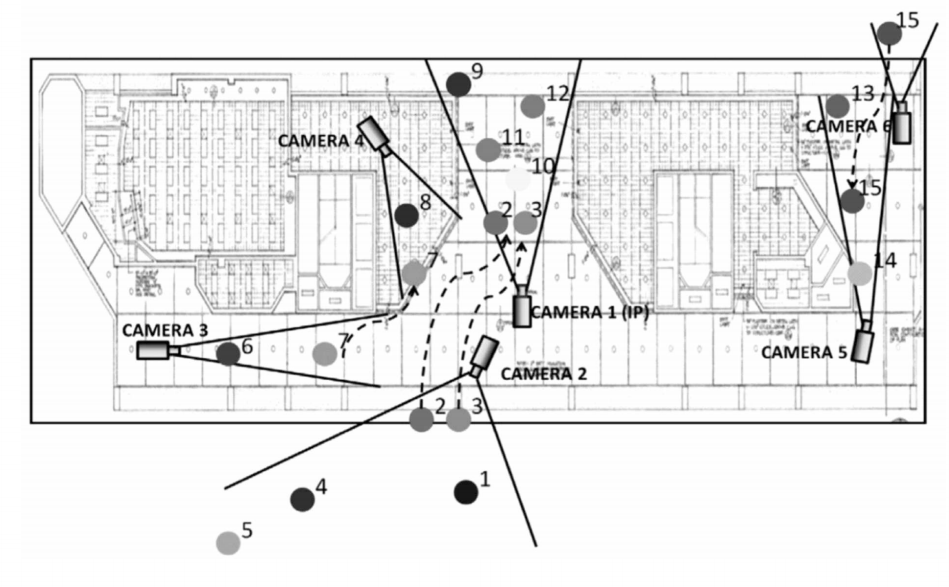
\includegraphics[width=0.75\linewidth]{2018-03-07-19-33-13.png}
	\end{figure}
	\note{
		随着监控摄像机的大规模安装,摄像机网络已广泛布控于各种公共场合中。
		
		利用摄像机网络,我们可以追踪同一行人的轨迹. 
		
		但是面对多
		路监控和海量的视频数据,监控人员很容易 疲惫和应接不暇 ,我们需要智能分析技术 来完成海量的工作
	}
\end{frame}


\begin{frame}
	{行人再识别定义}
	\begin{block}{前提假设}
		\begin{itemize}
			\item 检测器已经成功检测
			\item \ie, 再识别{\bf 不包括}检测步骤
		\end{itemize}
	% 输入某一行人的询问图片(Probe), 在图像或者视频集合(gallery)中跨摄像头检索所有包含该行人的图片. \cite{zheng2016person},\cite{Zheng2017person}
	\end{block}
	\begin{figure}
		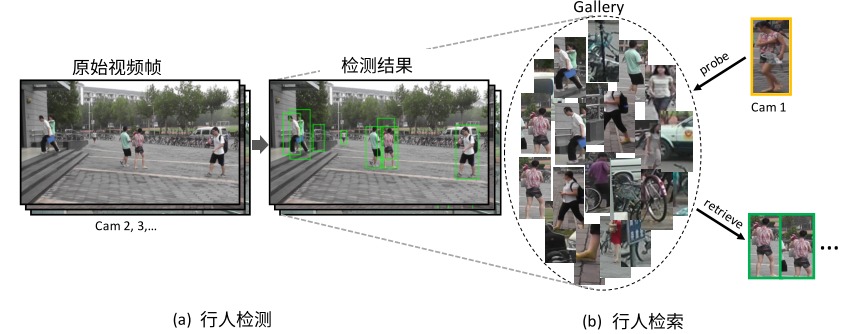
\includegraphics[width=1\linewidth]{background.png}
	\end{figure}
	\note{
		目前学术界几乎所有论文都采用这样的前提假设。行人再识别不包括行人检测的步骤。
		我们不讨论行人再识别的定义是否有问题,先遵循普遍接受的定义
	}
\end{frame}
		


\begin{frame}
	{行人再识别定义}
	\begin{block}{行人再识别 (Person Re-identification, \textit{aka.} ReID)}
		输入某一行人的询问图片(Probe), 在图像或者视频集合(gallery)中跨摄像头检索所有包含该行人的图片. 
	\end{block}
	\begin{columns}
		\column{0.3\textwidth} 
		\centering 
		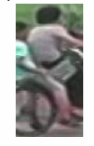
\includegraphics[width=0.5\linewidth]{2018-03-12-10-05-13.png}
		\column{0.7\textwidth} 
		\centering
		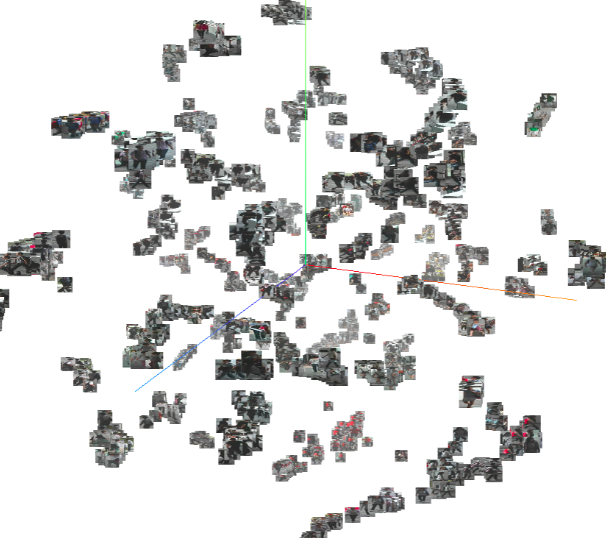
\includegraphics[width=0.72\linewidth]{2018-03-12-09-57-11.png}
	\end{columns}
	\note{
		行人再识别 是图像检索的子问题 , 他是这样的一个过称:
		
		输入询问图片,如左图所示,在右图测试图像集合中寻找最为匹配的行人图片

		匹配是指达到两点要求:1 两幅图属于同一个人,2 跨摄像头
	}
\end{frame}

\begin{frame}
	{行人再识别定义}
	\begin{block}{行人再识别 (Person Re-identification, \textit{aka.} ReID)}
		输入某一行人的询问图片(Probe), 在图像或者视频集合(gallery)中跨摄像头检索所有包含该行人的图片. 
	\end{block}
	\begin{figure}
		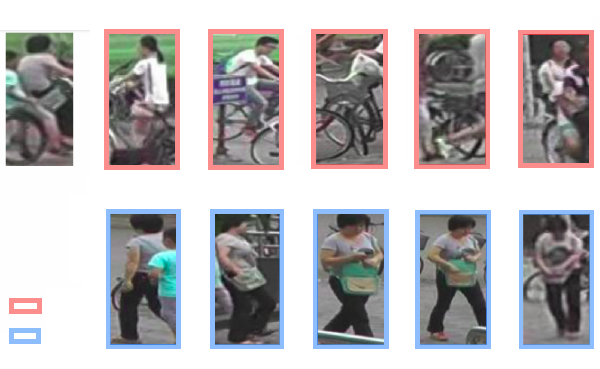
\includegraphics[width=0.9\linewidth]{2018-03-11-22-56-05.png}
	\end{figure}
	\note{
		为了说明再识别的困难,我挑选了模型预测的失败案例。
		
		左侧上方为预测结果,下防为期望的结果。由于询问蹄片特则不明显,测试集合存在大量干扰背景图片,模型的5个预测结果,军错误。背景干扰包括自信车、草地
	}
\end{frame}


\begin{frame}
	{存在的挑战}
	\begin{description}
		\item[Occlusion] 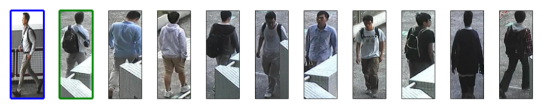
\includegraphics[width=0.9\linewidth]{2018-03-12-10-09-03.png}
		\item[Illumination] 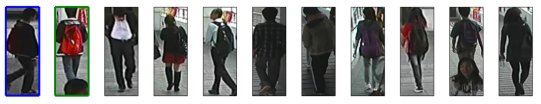
\includegraphics[width=0.9\linewidth]{2018-03-12-10-10-10.png}
		\item[Pose] 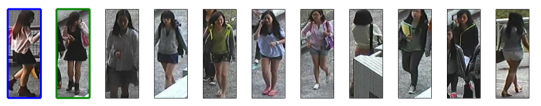
\includegraphics[width=0.9\linewidth]{2018-03-12-10-10-18.png}
		\item[Misalign] 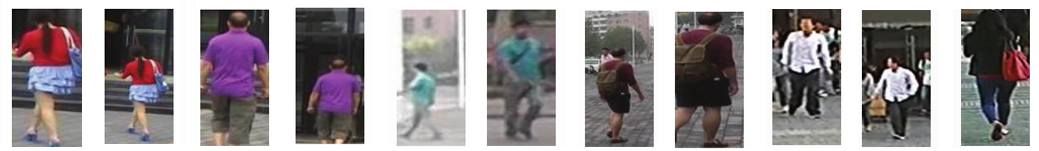
\includegraphics[width=0.88\linewidth]{2018-03-07-20-16-25.png}
	\end{description}
	
	\note{
		除背景干扰, 
		再识别的难点还有 遮挡、明暗、姿态倒置的行人外观巨大改变,以及由于检测器误差导致的空间适配。
	}
\end{frame}

\section{技术路线与设计方案}

\subsection{注意力机制}

\begin{frame}{动机}
	
\end{frame}

\subsection{度量学习}

\section{思考与展望}

\begin{frame}[t, allowframebreaks]
	\frametitle{参考文献}
	\printbibliography
\end{frame}

\begin{frame}
	\chuhao Thank you! %\fontspec{LHANDW.TTF}
\end{frame}


\begin{frame}[fragile]
	\frametitle{eval protocol}
\begin{lstlisting}
cmc_configs = {
'cuhk03': dict(separate_camera_set=True,
  single_gallery_shot=True,
  first_match_break=False),
'market1501': dict(separate_camera_set=False,#h
  single_gallery_shot=False,  # hard
  first_match_break=True),
'allshots': dict(separate_camera_set=False,#h
  single_gallery_shot=False,  # hard
  first_match_break=False),
}
\end{lstlisting}
\end{frame}

\end{document}
